\documentclass[12pt]{article}

\usepackage{tabularx}
\usepackage[a4paper,margin=2.5cm, bottom=2.5cm]{geometry}
\usepackage{fancyhdr}
\usepackage{listings}
\usepackage{booktabs}
\usepackage{float}
\usepackage{subcaption}
% \usepackage{caption}
% \captionsetup{font=footnotesize}
\usepackage{graphicx}
\usepackage{amsmath}
\usepackage{amssymb}
\usepackage{amsthm}
\usepackage{array}
\usepackage[table]{xcolor}
\usepackage{pgfplots}
\pgfplotsset{compat=1.17}
\usepackage{pgfplotstable}
\usepackage{multirow}
\usepackage{tikz}
\usepackage[hidelinks]{hyperref}
\usepackage{titling}
\usepackage[polish]{babel} % Polish language support

\setlength{\headheight}{40pt}
\setlength{\parindent}{0pt}
\setlength{\parskip}{1ex}
\renewcommand{\headrulewidth}{0pt}

\pagestyle{fancy}
\fancyhead{}
\fancyhead[L]{
    \renewcommand{\arraystretch}{1.5}
    \begin{tabularx}{\textwidth}{|X|X|}
        \hline
        \bfseries Obliczenia inteligentne & \bfseries \thetitle \\
        \hline
    \end{tabularx}
}
\fancyfoot[C]{\thepage}

\renewcommand{\maketitle}{
    \thispagestyle{plain}
    \renewcommand{\arraystretch}{2}
    \vspace*{-8em}
    \footnotesize
    \begin{flushleft}
        \begin{tabularx}{\textwidth}{|X|X|}
            \hline
            \bfseries Obliczenia Inteligentne  & \bfseries \thetitle                           \\ \hline
            \multicolumn{2}{|l|}{
                \begin{tabular}[t]{@{}ll@{}} 
                    \textbf{Grupa:} Grupa 1
                    \hspace{4.5em}
                    \textbf{Dzień i czas:} Czwartek, 10:00
                    \hspace{4.5em}
                    \textbf{Rok akademicki:} 2023/24
                \end{tabular}
            } \\ \hline
            \multicolumn{2}{|l|}{
                \begin{tabular}[t]{@{}l@{\hspace{10em}}l@{}} 
                    \textbf{Imię i nazwisko:} \textsc{Jakub Pawlak} & \textbf{Imię i nazwisko:} \textsc{Magdalena Paku\l a} 
                \end{tabular}
            } \\
            \hline
        \end{tabularx}
    \end{flushleft}
    \renewcommand{\arraystretch}{1}
}


\title{Projekt 1}


\begin{document}
\maketitle

% PIERWSZA STRONA
\section{Eksperyment 1: Metoda K-Means}
\vspace{-1em}
% Wyniki dla Sztucznie Wygenerowanych Zbiorów Danych
\begin{figure}[H]
    \centering
    \begin{subfigure}[b]{0.3\textwidth}
        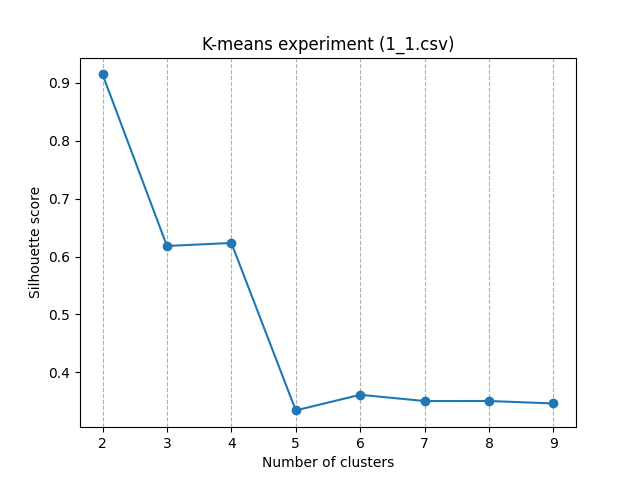
\includegraphics[width=\linewidth]{img/exp_1/kmeans/1_1_scores.png}
        \caption{Zbior 1\_1}
    \end{subfigure}
    \hfill
    \begin{subfigure}[b]{0.3\textwidth}
        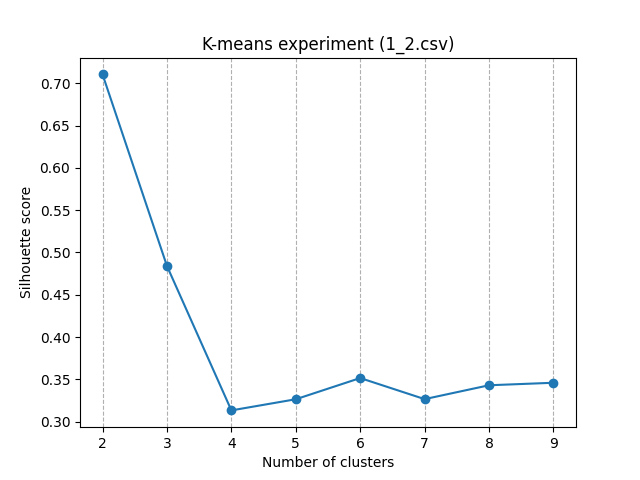
\includegraphics[width=\linewidth]{img/exp_1/kmeans/1_2_scores.png}
        \caption{Zbior 1\_2}
    \end{subfigure}
    \hfill
    \begin{subfigure}[b]{0.3\textwidth}
        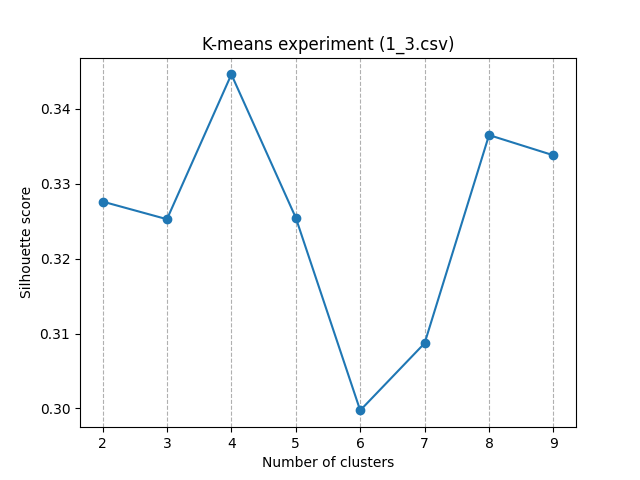
\includegraphics[width=\linewidth]{img/exp_1/kmeans/1_3_scores.png}
        \caption{Zbior 1\_3}
    \end{subfigure}
    \begin{subfigure}[b]{0.3\textwidth}
        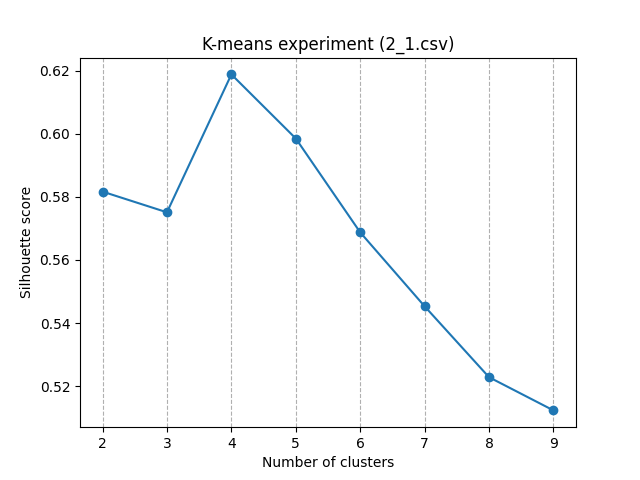
\includegraphics[width=\linewidth]{img/exp_1/kmeans/2_1_scores.png}
        \caption{Zbior 2\_1}
    \end{subfigure}
    \hfill
    \begin{subfigure}[b]{0.3\textwidth}
        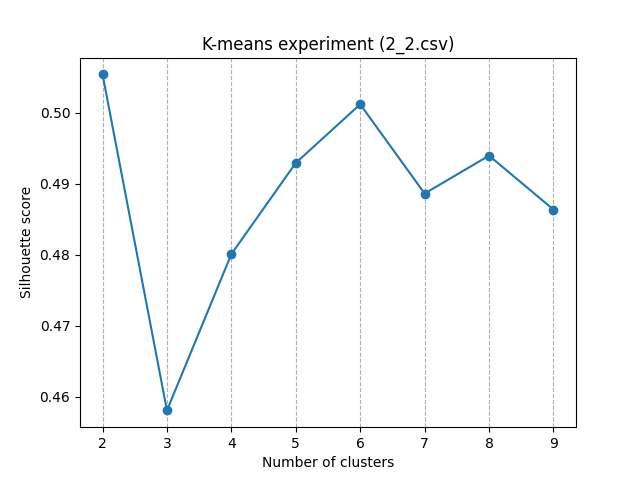
\includegraphics[width=\linewidth]{img/exp_1/kmeans/2_2_scores.png}
        \caption{Zbior 2\_2}
    \end{subfigure}
    \hfill
    \begin{subfigure}[b]{0.3\textwidth}
        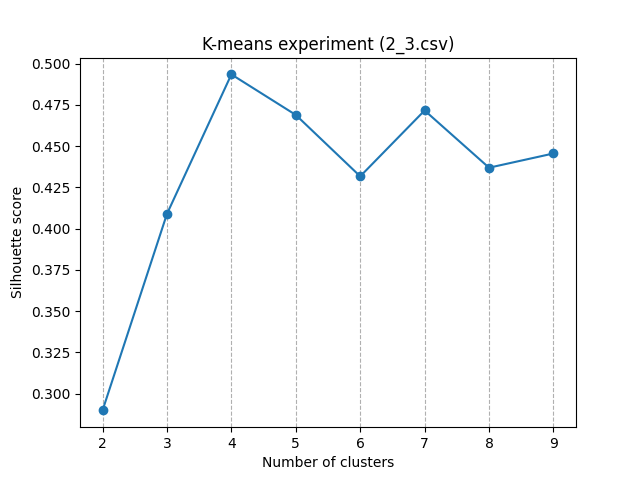
\includegraphics[width=\linewidth]{img/exp_1/kmeans/2_3_scores.png}
        \caption{Zbior 2\_3}
    \end{subfigure}
    \caption{\centering Zmiana wartości silhouette score dla wszystkich zbiorów w zależności od parametru n\_clusters w metodzie K-means}
\end{figure}

% Najlepszy i najgorszy przypadek dla wszystkich zbiorów
\begin{figure}[H]
    \centering
    \begin{subfigure}[b]{0.24\textwidth}
        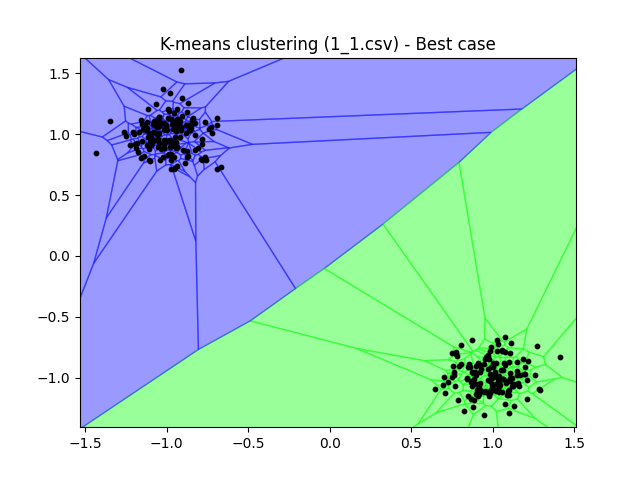
\includegraphics[width=\linewidth]{img/exp_1/kmeans/1_1_best.png}
        \caption{Najlepszy dla 1\_1}
    \end{subfigure}
    \hfill
    \begin{subfigure}[b]{0.24\textwidth}
        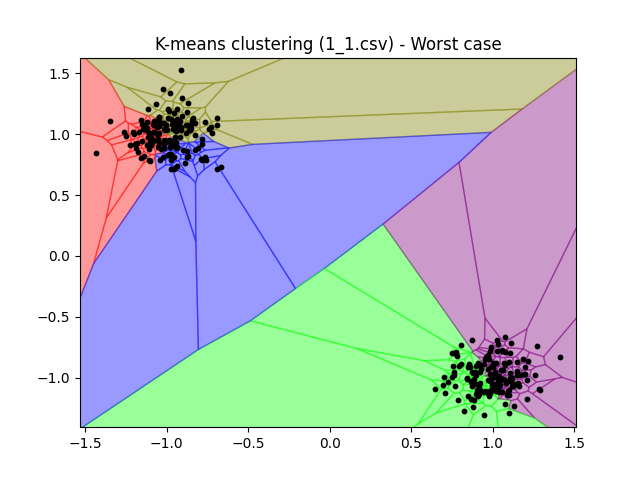
\includegraphics[width=\linewidth]{img/exp_1/kmeans/1_1_worst.png}
        \caption{Najgorszy dla 1\_1}
    \end{subfigure}
    \hfill
    \begin{subfigure}[b]{0.24\textwidth}
        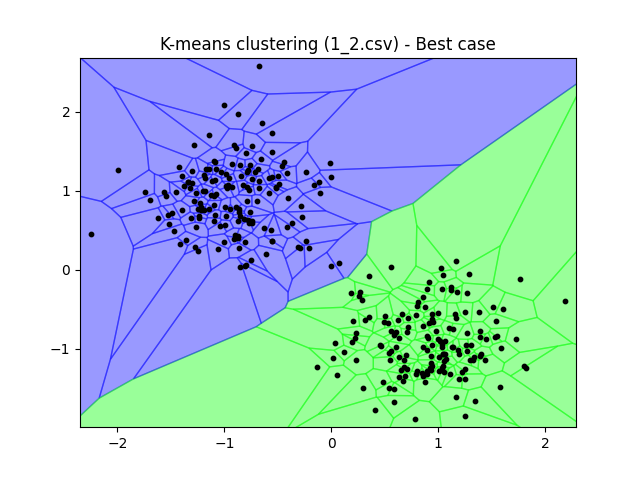
\includegraphics[width=\linewidth]{img/exp_1/kmeans/1_2_best.png}
        \caption{Najlepszy dla 1\_2}
    \end{subfigure}
    \hfill
    \begin{subfigure}[b]{0.24\textwidth}
        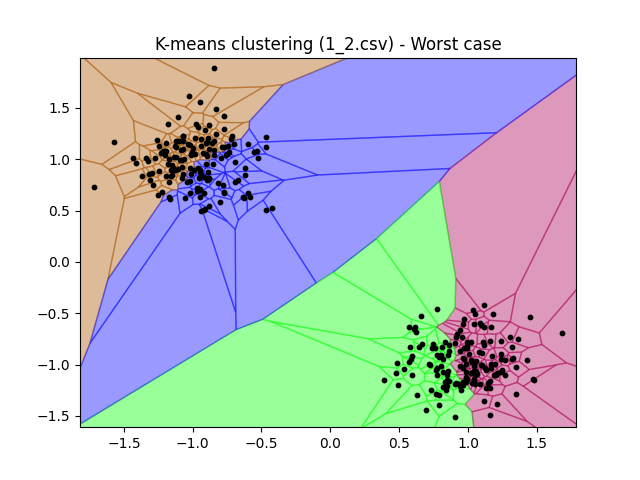
\includegraphics[width=\linewidth]{img/exp_1/kmeans/1_2_worst.png}
        \caption{Najgorszy dla 1\_2}
    \end{subfigure}
    \begin{subfigure}[b]{0.24\textwidth}
        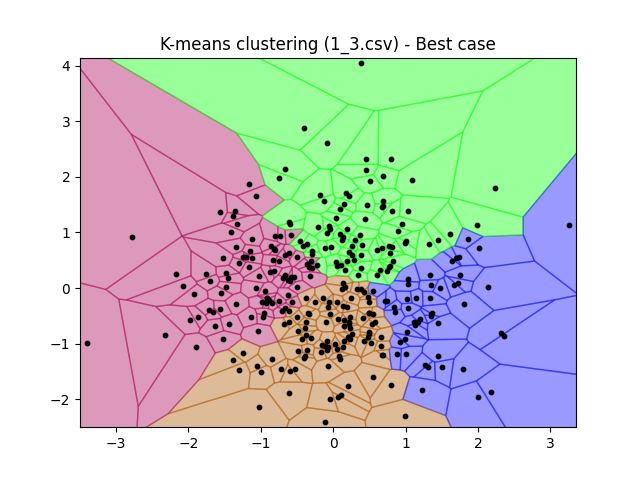
\includegraphics[width=\linewidth]{img/exp_1/kmeans/1_3_best.png}
        \caption{Najlepszy dla 1\_3}
    \end{subfigure}
    \hfill
    \begin{subfigure}[b]{0.24\textwidth}
        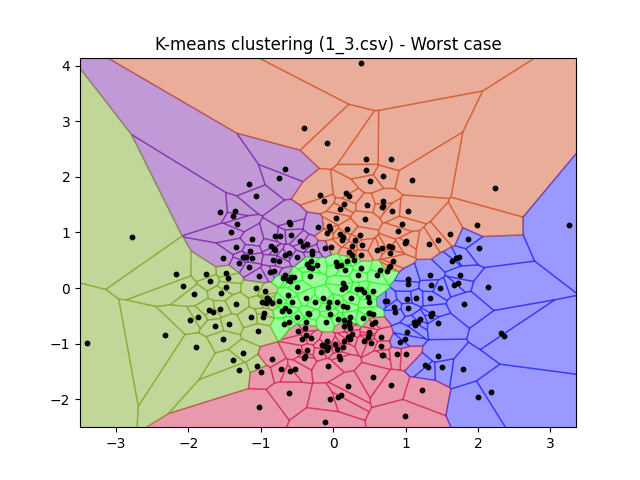
\includegraphics[width=\linewidth]{img/exp_1/kmeans/1_3_worst.png}
        \caption{Najgorszy dla 1\_3}
    \end{subfigure}
    \hfill
    \begin{subfigure}[b]{0.24\textwidth}
        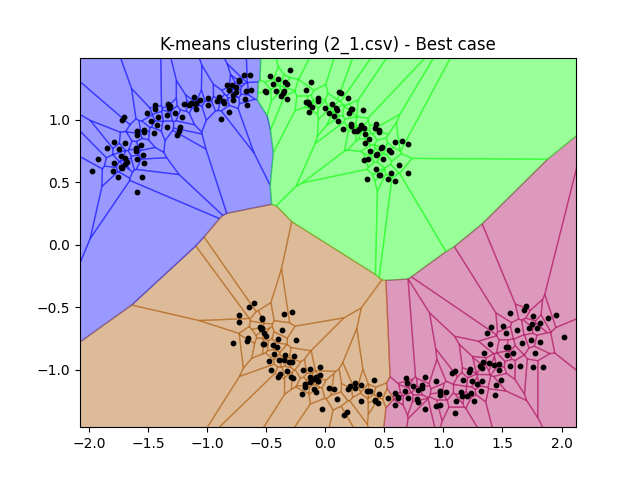
\includegraphics[width=\linewidth]{img/exp_1/kmeans/2_1_best.png}
        \caption{Najlepszy dla 2\_1}
    \end{subfigure}
    \hfill
    \begin{subfigure}[b]{0.24\textwidth}
        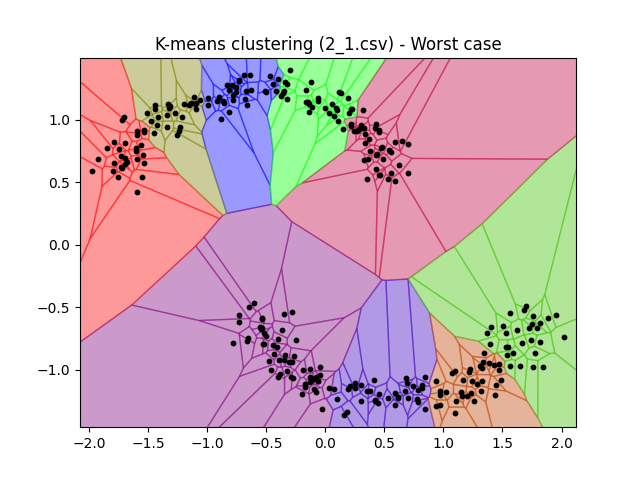
\includegraphics[width=\linewidth]{img/exp_1/kmeans/2_1_worst.png}
        \caption{Najgorszy dla 2\_1}
    \end{subfigure}
    \begin{subfigure}[b]{0.24\textwidth}
        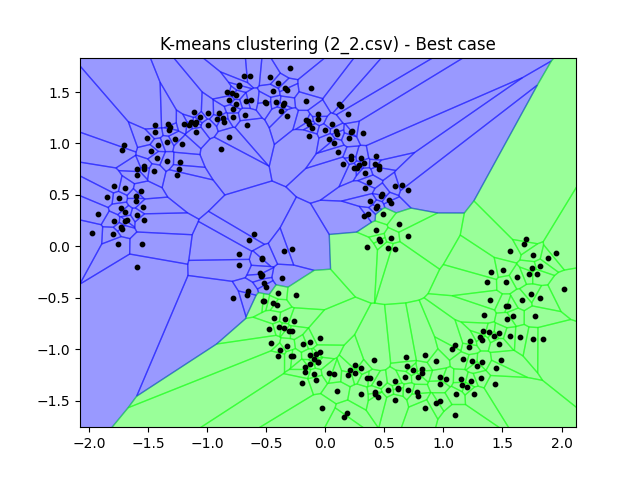
\includegraphics[width=\linewidth]{img/exp_1/kmeans/2_2_best.png}
        \caption{Najlepszy dla 2\_2}
    \end{subfigure}
    \hfill
    \begin{subfigure}[b]{0.24\textwidth}
        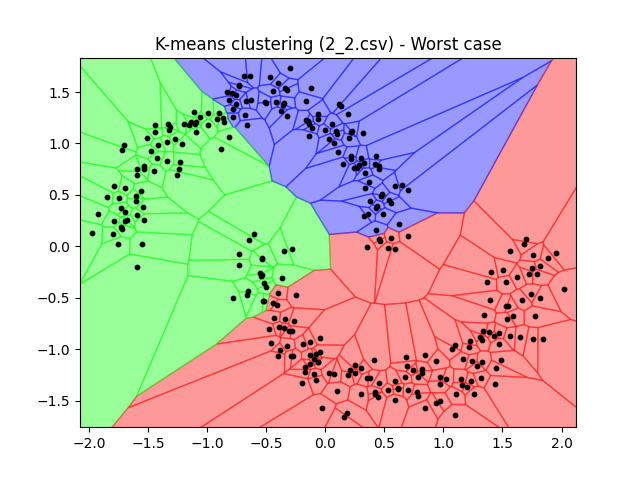
\includegraphics[width=\linewidth]{img/exp_1/kmeans/2_2_worst.png}
        \caption{Najgorszy dla 2\_2}
    \end{subfigure}
    \hfill
    \begin{subfigure}[b]{0.24\textwidth}
        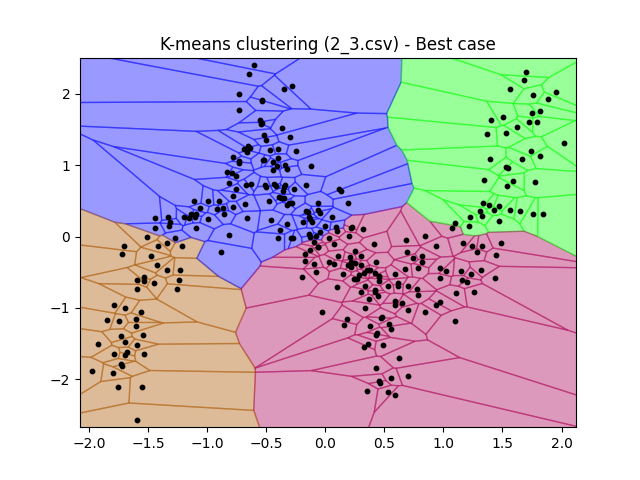
\includegraphics[width=\linewidth]{img/exp_1/kmeans/2_3_best.png}
        \caption{Najlepszy dla 2\_3}
    \end{subfigure}
    \hfill
    \begin{subfigure}[b]{0.24\textwidth}
        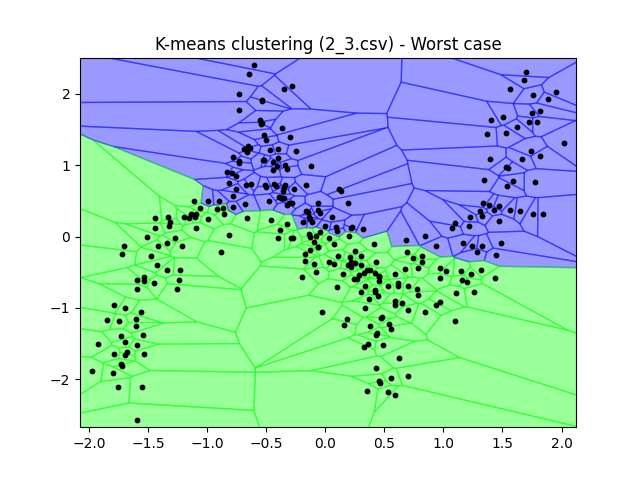
\includegraphics[width=\linewidth]{img/exp_1/kmeans/2_3_worst.png}
        \caption{Najgorszy dla 2\_3}
    \end{subfigure}
    \caption{\centering Wizualizacja klastrów dla wszystkich zbiorów na diagramie Voronoia dla najlepszego i najgorszego przypadku w metodzie K-means}
\end{figure}

\pagebreak
% DRUGA STRONA
\section{Eksperyment 1: Metoda DBSCAN}
% Wyniki dla Sztucznie Wygenerowanych Zbiorów Danych
\begin{figure}[H]
    \centering
    \begin{subfigure}[b]{0.3\textwidth}
        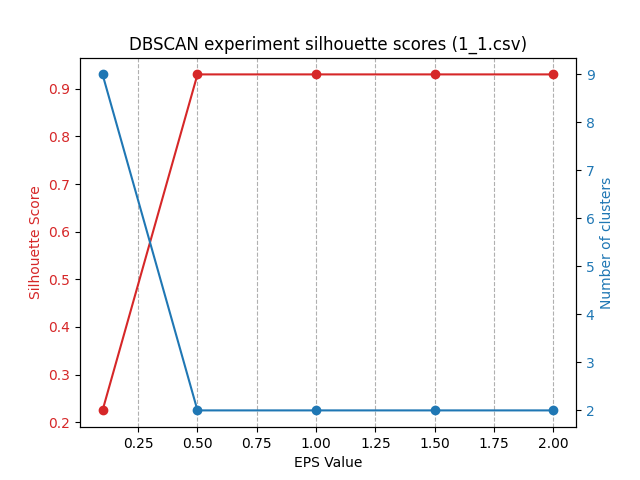
\includegraphics[width=\linewidth]{img/exp_1/dbscan/1_1_scores.png}
        \caption{Zbior 1\_1}
    \end{subfigure}
    \hfill
    \begin{subfigure}[b]{0.3\textwidth}
        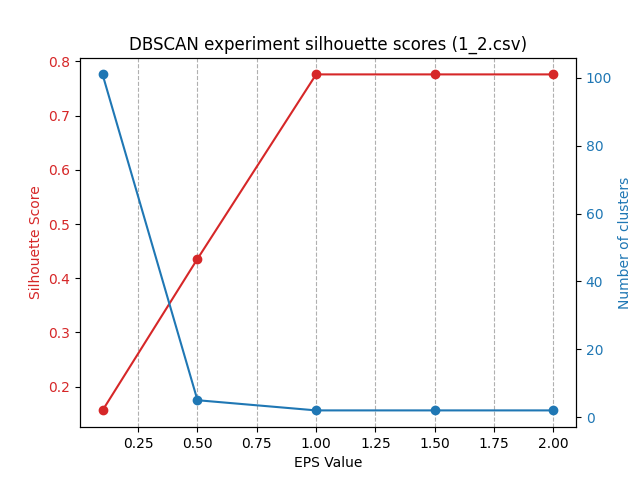
\includegraphics[width=\linewidth]{img/exp_1/dbscan/1_2_scores.png}
        \caption{Zbior 1\_2}
    \end{subfigure}
    \hfill
    \begin{subfigure}[b]{0.3\textwidth}
        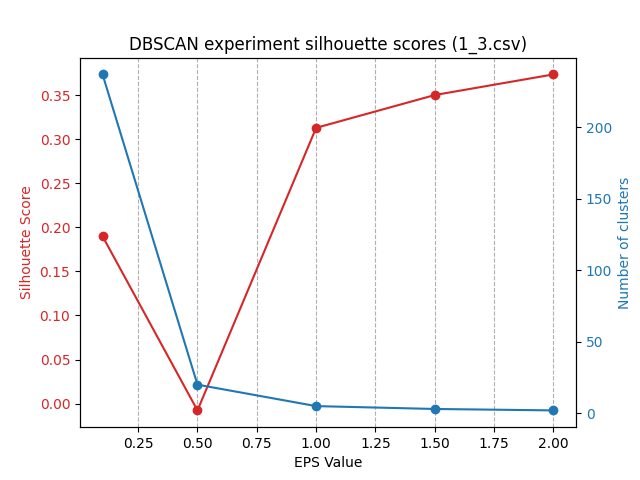
\includegraphics[width=\linewidth]{img/exp_1/dbscan/1_3_scores.png}
        \caption{Zbior 1\_3}
    \end{subfigure}
    \begin{subfigure}[b]{0.3\textwidth}
        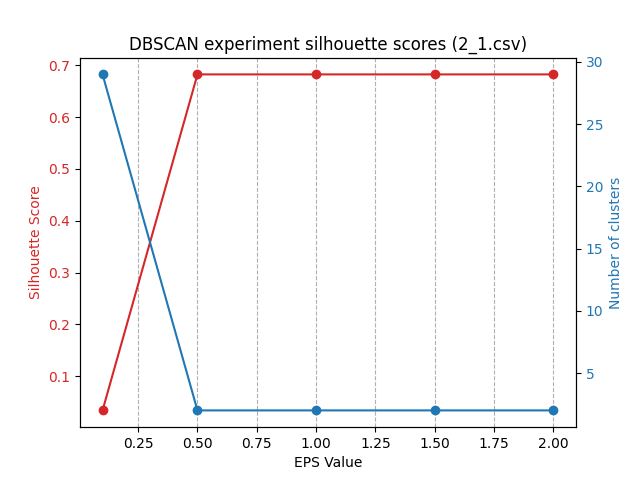
\includegraphics[width=\linewidth]{img/exp_1/dbscan/2_1_scores.png}
        \caption{Zbior 2\_1}
    \end{subfigure}
    \hfill
    \begin{subfigure}[b]{0.3\textwidth}
        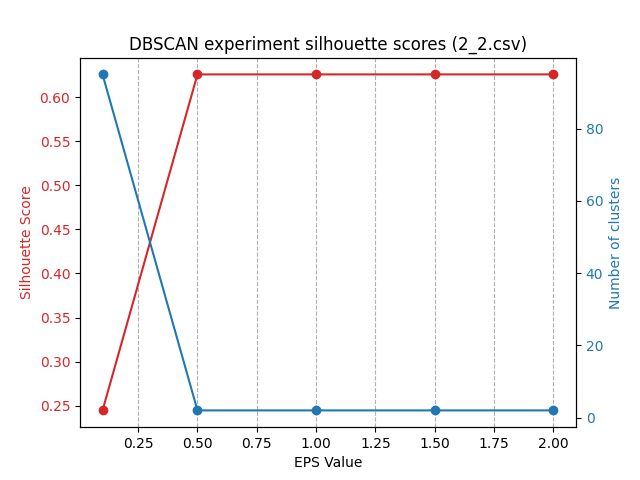
\includegraphics[width=\linewidth]{img/exp_1/dbscan/2_2_scores.png}
        \caption{Zbior 2\_2}
    \end{subfigure}
    \hfill
    \begin{subfigure}[b]{0.3\textwidth}
        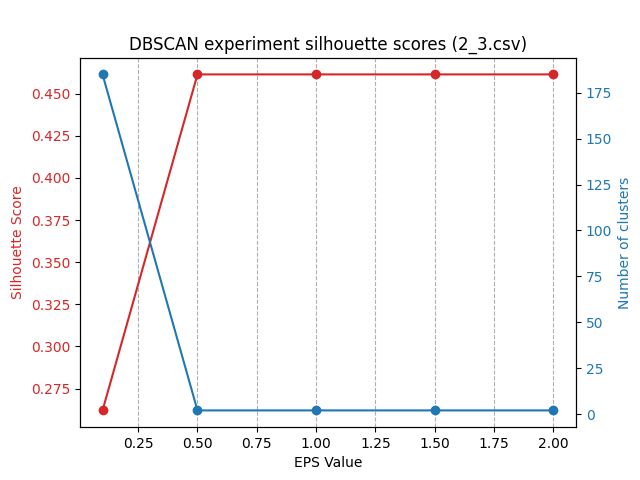
\includegraphics[width=\linewidth]{img/exp_1/dbscan/2_3_scores.png}
        \caption{Zbior 2\_3}
    \end{subfigure}
    \caption{\centering Zmiana wartości silhouette score oraz n\_clusters dla wszystkich zbiorów w zależności od zmieniającego się parametru eps w metodzie DBSCAN}
\end{figure}

% Najlepszy i najgorszy przypadek dla wszystkich zbiorów
\begin{figure}[H]
    \centering
    \begin{subfigure}[b]{0.24\textwidth}
        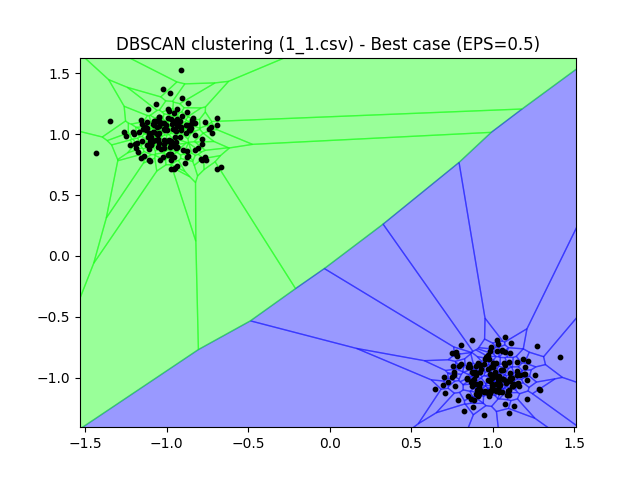
\includegraphics[width=\linewidth]{img/exp_1/dbscan/1_1_best.png}
        \caption{Najlepszy dla 1\_1}
    \end{subfigure}
    \hfill
    \begin{subfigure}[b]{0.24\textwidth}
        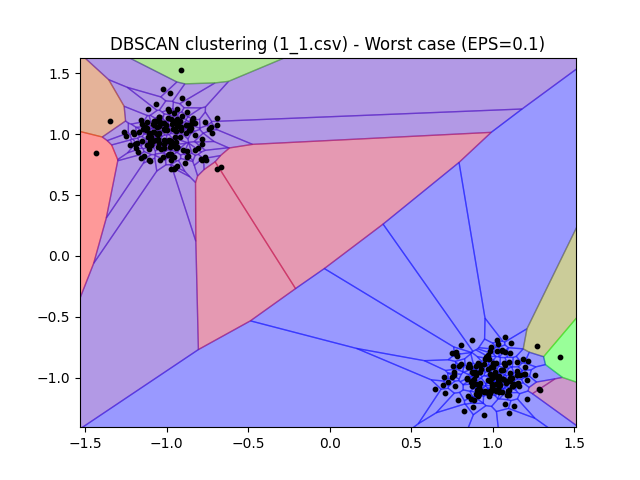
\includegraphics[width=\linewidth]{img/exp_1/dbscan/1_1_worst.png}
        \caption{Najgorszy dla 1\_1}
    \end{subfigure}
    \hfill
    \begin{subfigure}[b]{0.24\textwidth}
        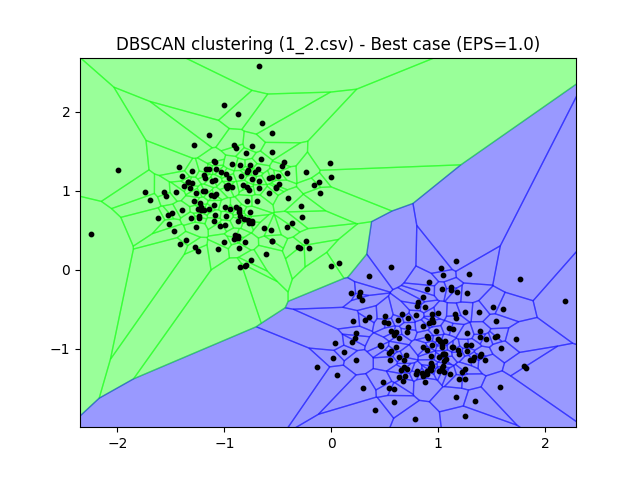
\includegraphics[width=\linewidth]{img/exp_1/dbscan/1_2_best.png}
        \caption{Najlepszy dla 1\_2}
    \end{subfigure}
    \hfill
    \begin{subfigure}[b]{0.24\textwidth}
        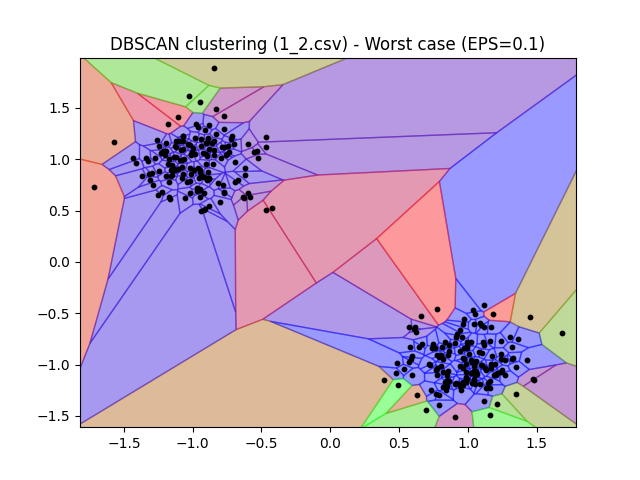
\includegraphics[width=\linewidth]{img/exp_1/dbscan/1_2_worst.png}
        \caption{Najgorszy dla 1\_2}
    \end{subfigure}
    \begin{subfigure}[b]{0.24\textwidth}
        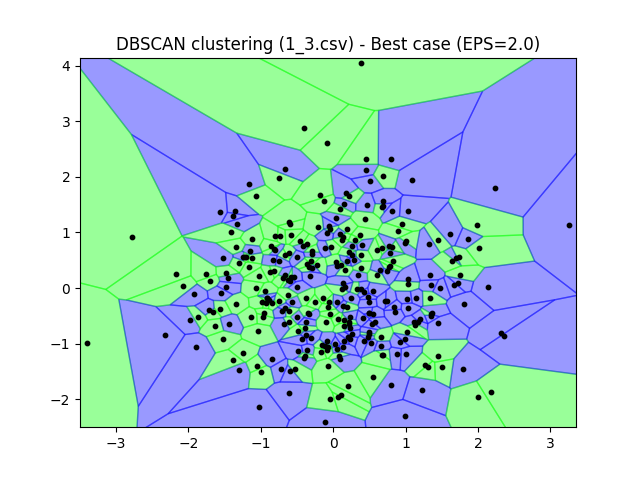
\includegraphics[width=\linewidth]{img/exp_1/dbscan/1_3_best.png}
        \caption{Najlepszy dla 1\_3}
    \end{subfigure}
    \hfill
    \begin{subfigure}[b]{0.24\textwidth}
        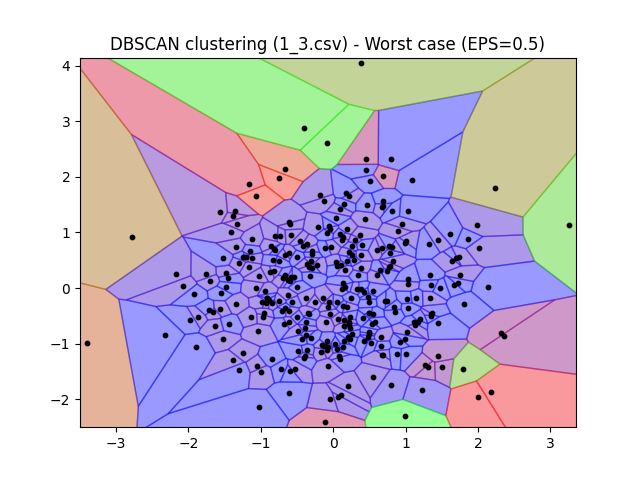
\includegraphics[width=\linewidth]{img/exp_1/dbscan/1_3_worst.png}
        \caption{Najgorszy dla 1\_3}
    \end{subfigure}
    \hfill
    \begin{subfigure}[b]{0.24\textwidth}
        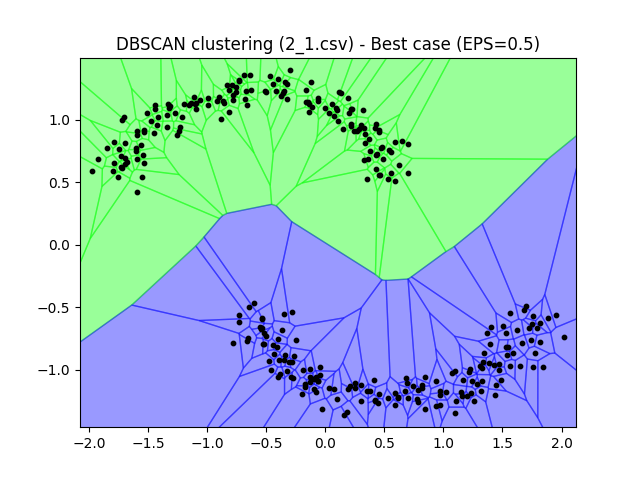
\includegraphics[width=\linewidth]{img/exp_1/dbscan/2_1_best.png}
        \caption{Najlepszy dla 2\_1}
    \end{subfigure}
    \hfill
    \begin{subfigure}[b]{0.24\textwidth}
        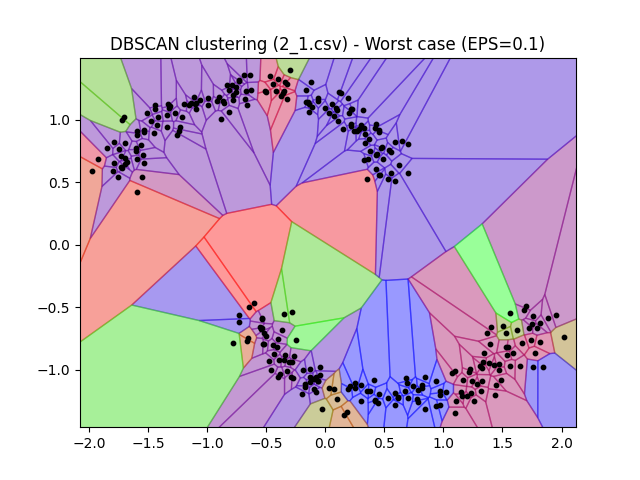
\includegraphics[width=\linewidth]{img/exp_1/dbscan/2_1_worst.png}
        \caption{Najgorszy dla 2\_1}
    \end{subfigure}
    \begin{subfigure}[b]{0.24\textwidth}
        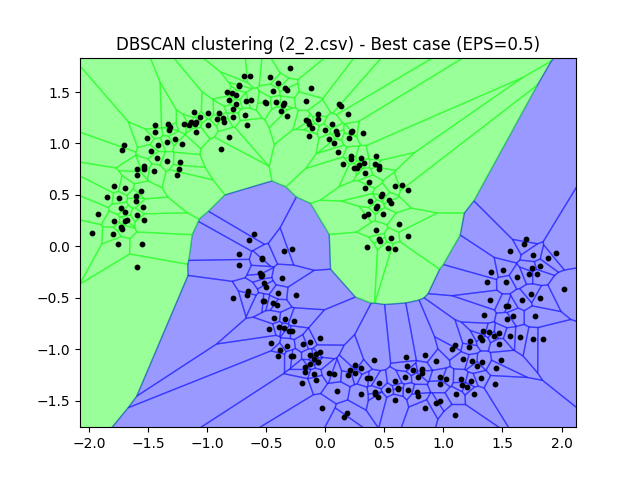
\includegraphics[width=\linewidth]{img/exp_1/dbscan/2_2_best.png}
        \caption{Najlepszy dla 2\_2}
    \end{subfigure}
    \hfill
    \begin{subfigure}[b]{0.24\textwidth}
        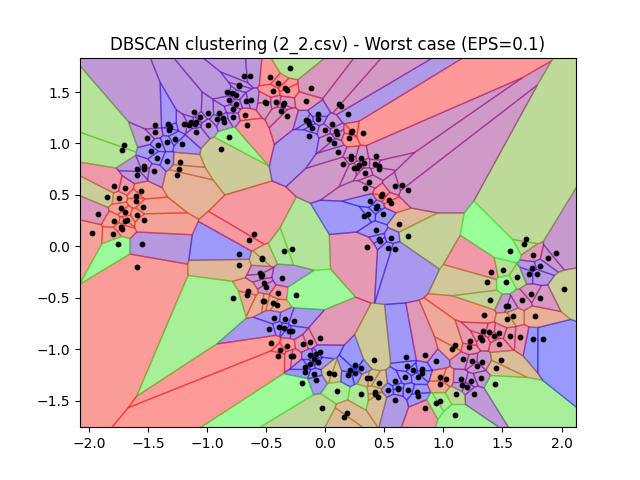
\includegraphics[width=\linewidth]{img/exp_1/dbscan/2_2_worst.png}
        \caption{Najgorszy dla 2\_2}
    \end{subfigure}
    \hfill
    \begin{subfigure}[b]{0.24\textwidth}
        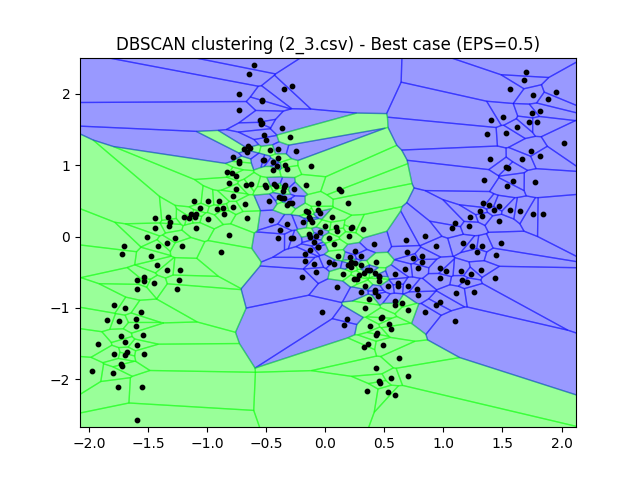
\includegraphics[width=\linewidth]{img/exp_1/dbscan/2_3_best.png}
        \caption{Najlepszy dla 2\_3}
    \end{subfigure}
    \hfill
    \begin{subfigure}[b]{0.24\textwidth}
        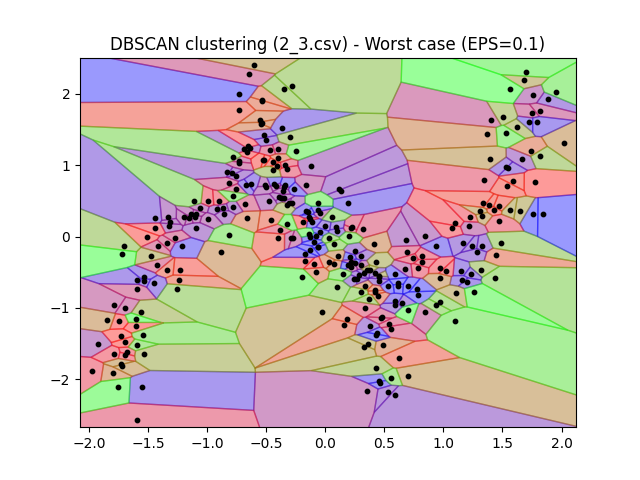
\includegraphics[width=\linewidth]{img/exp_1/dbscan/2_3_worst.png}
        \caption{Najgorszy dla 2\_3}
    \end{subfigure}
    \caption{\centering Wizualizacja klastrów dla wszystkich zbiorów na diagramie Voronoia dla najlepszego i najgorszego przypadku w metodzie DBSCAN}
\end{figure}

% TRZECIA STRONA
\section{Eksperyment 2: Metoda K-Means z etykietami}

% Wyniki drugiego eksperymentu dla sześciu sztucznie wygenerowanych zbiorów danych i metody K-Means.
% Dla każdego zbioru należy pokazać wykres obrazujący zmianę wartości miar adjusted rand score, homogeneity score,  completeness score oraz V-measure score przy zmieniającym się parametrze n-clusters oraz wizualizację klastrów (diagram Woronoja z pokazanymi prawdziwymi etykietami obiektów) dla najlepszego i najgorszego przypadku (wskazując, który to był przypadek i dlaczego).

\begin{figure}[H]
    \centering
    \begin{subfigure}[b]{0.3\textwidth}
        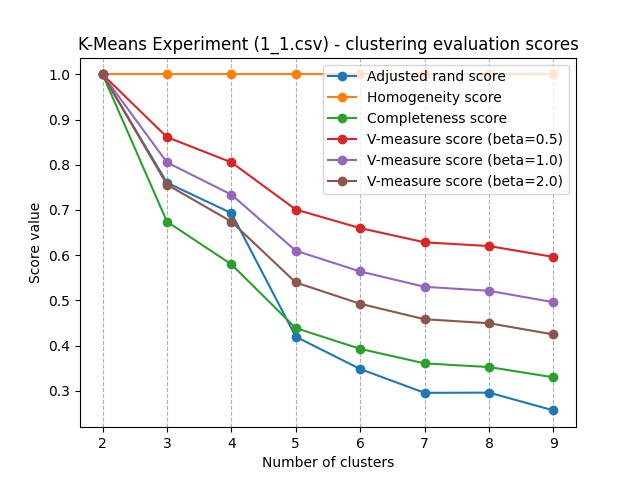
\includegraphics[width=\linewidth]{img/exp_2/kmeans/1_1_scores.png}
        \caption{Zbior 1\_1}
    \end{subfigure}
    \hfill
    \begin{subfigure}[b]{0.3\textwidth}
        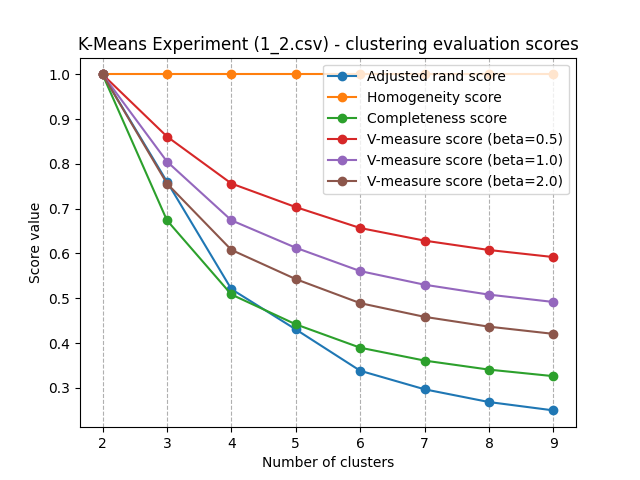
\includegraphics[width=\linewidth]{img/exp_2/kmeans/1_2_scores.png}
        \caption{Zbior 1\_2}
    \end{subfigure}
    \hfill
    \begin{subfigure}[b]{0.3\textwidth}
        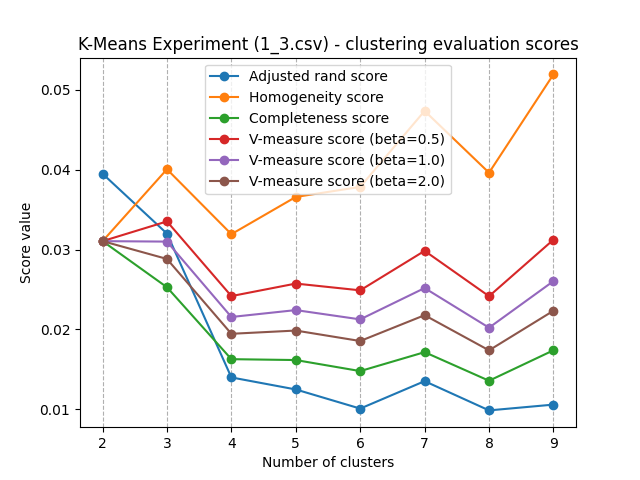
\includegraphics[width=\linewidth]{img/exp_2/kmeans/1_3_scores.png}
        \caption{Zbior 1\_3}
    \end{subfigure}
    \begin{subfigure}[b]{0.3\textwidth}
        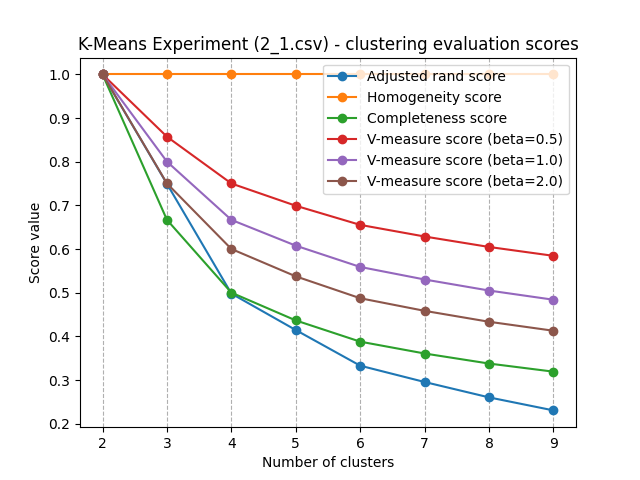
\includegraphics[width=\linewidth]{img/exp_2/kmeans/2_1_scores.png}
        \caption{Zbior 2\_1}
    \end{subfigure}
    \hfill
    \begin{subfigure}[b]{0.3\textwidth}
        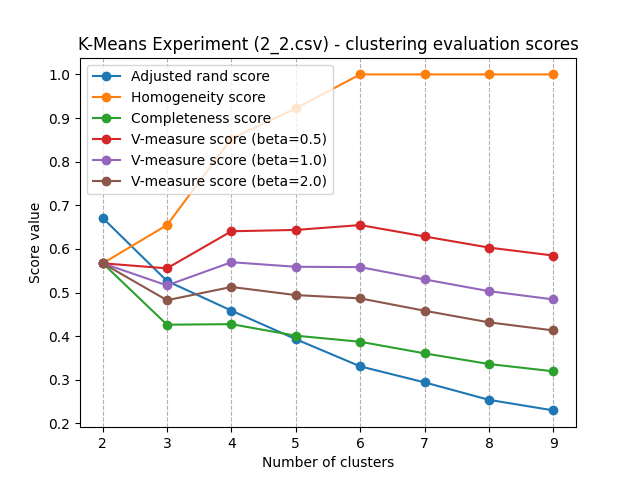
\includegraphics[width=\linewidth]{img/exp_2/kmeans/2_2_scores.png}
        \caption{Zbior 2\_2}
    \end{subfigure}
    \hfill
    \begin{subfigure}[b]{0.3\textwidth}
        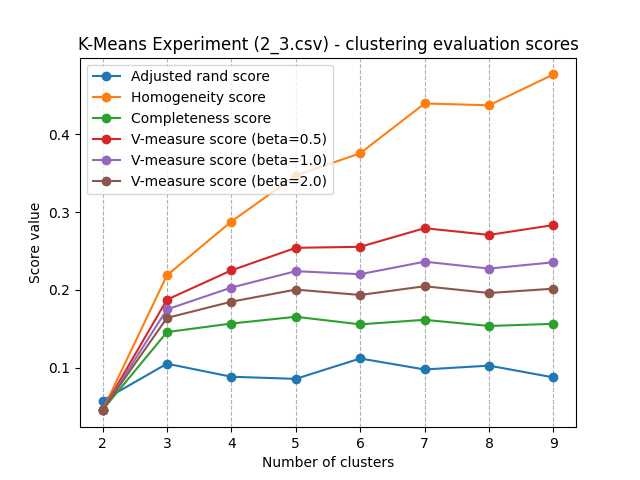
\includegraphics[width=\linewidth]{img/exp_2/kmeans/2_3_scores.png}
        \caption{Zbior 2\_3}
    \end{subfigure}
    \caption{\centering Zmiana wartości miar jakosći dla wszystkich zbiorów w zależności od liczby klastrów w metodzie K-means}
\end{figure}

\begin{figure}[H]
    \centering
    \begin{subfigure}[b]{0.24\textwidth}
        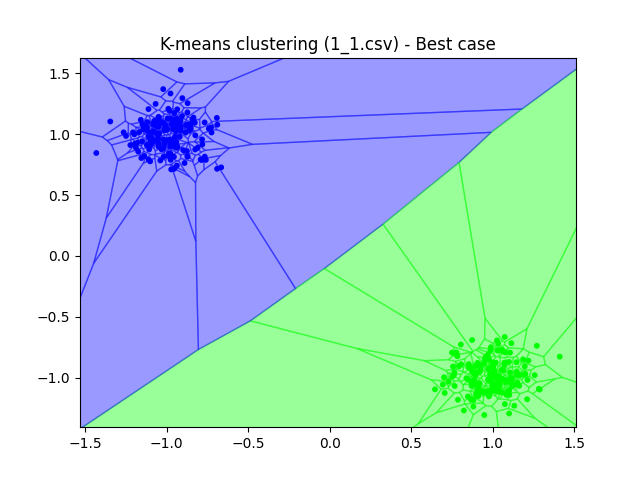
\includegraphics[width=\linewidth]{img/exp_2/kmeans/1_1_best.png}
        \caption{Najlepszy dla 1\_1}
    \end{subfigure}
    \hfill
    \begin{subfigure}[b]{0.24\textwidth}
        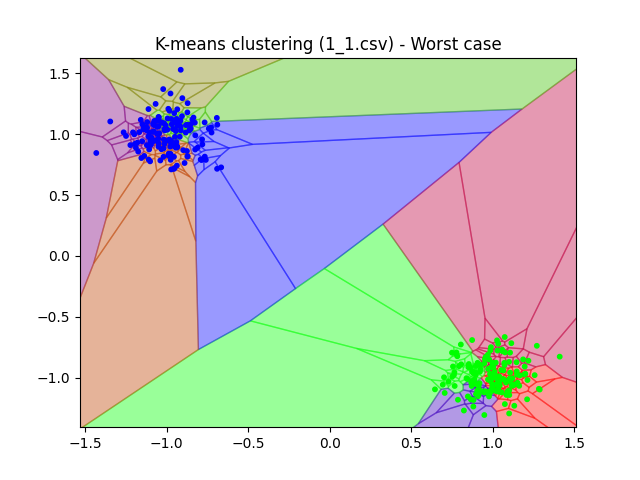
\includegraphics[width=\linewidth]{img/exp_2/kmeans/1_1_worst.png}
        \caption{Najgorszy dla 1\_1}
    \end{subfigure}
    \hfill
    \begin{subfigure}[b]{0.24\textwidth}
        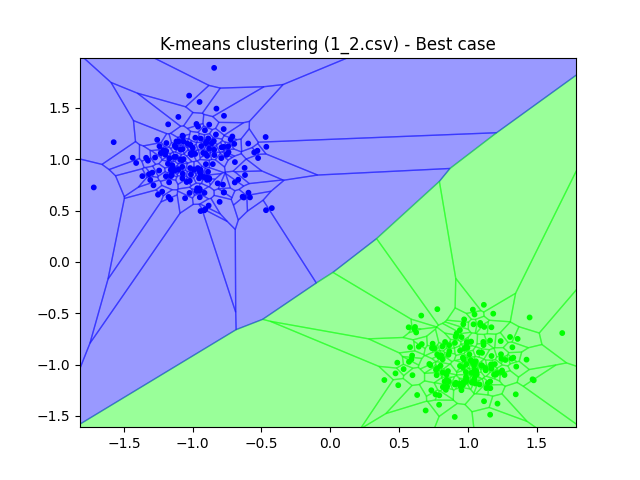
\includegraphics[width=\linewidth]{img/exp_2/kmeans/1_2_best.png}
        \caption{Najlepszy dla 1\_2}
    \end{subfigure}
    \hfill
    \begin{subfigure}[b]{0.24\textwidth}
        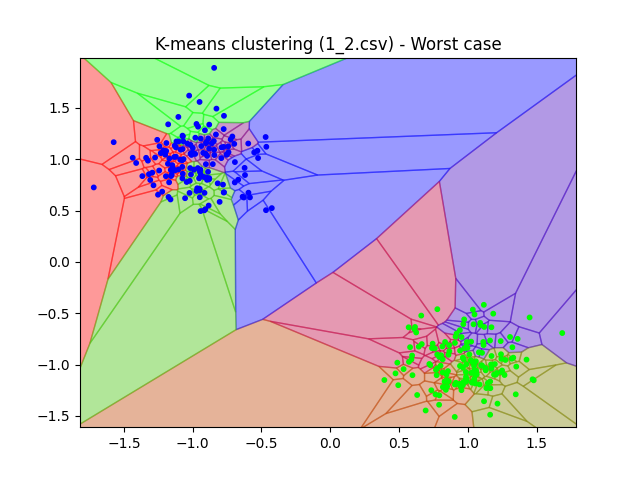
\includegraphics[width=\linewidth]{img/exp_2/kmeans/1_2_worst.png}
        \caption{Najgorszy dla 1\_2}
    \end{subfigure}
    \begin{subfigure}[b]{0.24\textwidth}
        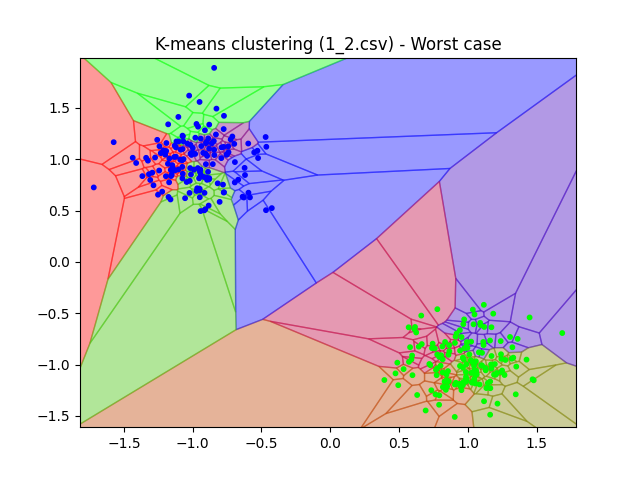
\includegraphics[width=\linewidth]{img/exp_2/kmeans/1_2_worst.png}
        \caption{Najlepszy dla 1\_3}
    \end{subfigure}
    \hfill
    \begin{subfigure}[b]{0.24\textwidth}
        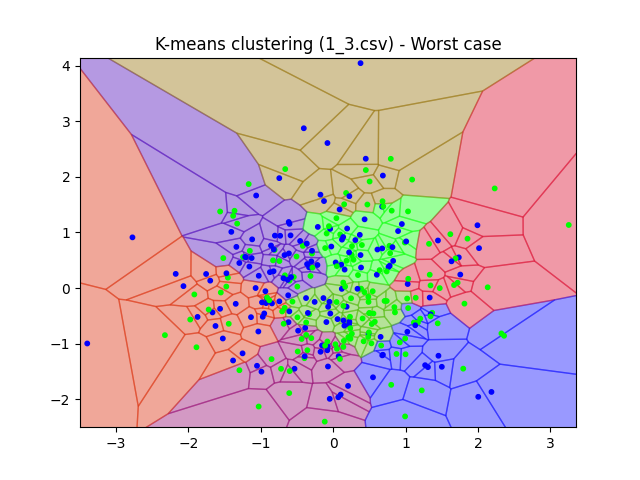
\includegraphics[width=\linewidth]{img/exp_2/kmeans/1_3_worst.png}
        \caption{Najgorszy dla 1\_3}
    \end{subfigure}
    \hfill
    \begin{subfigure}[b]{0.24\textwidth}
        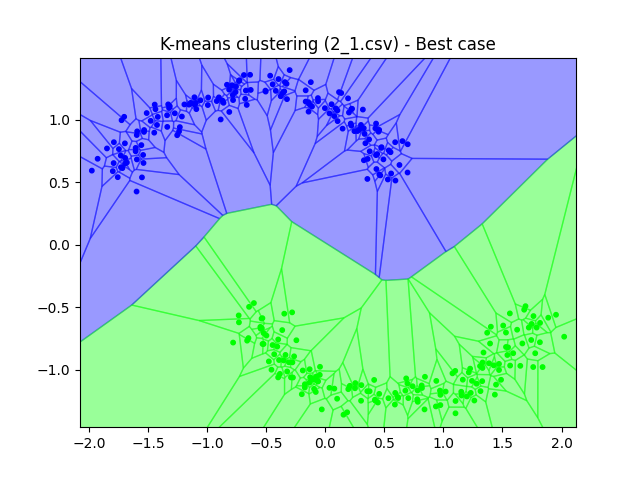
\includegraphics[width=\linewidth]{img/exp_2/kmeans/2_1_best.png}
        \caption{Najlepszy dla 2\_1}
    \end{subfigure}
    \hfill
    \begin{subfigure}[b]{0.24\textwidth}
        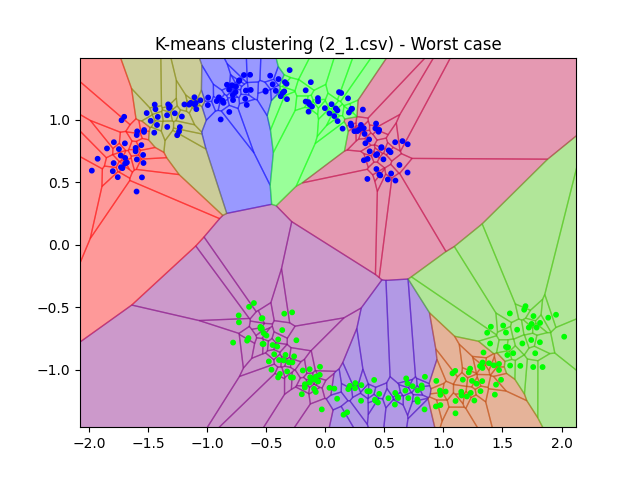
\includegraphics[width=\linewidth]{img/exp_2/kmeans/2_1_worst.png}
        \caption{Najgorszy dla 2\_1}
    \end{subfigure}
    \begin{subfigure}[b]{0.24\textwidth}
        \includegraphics[width=\linewidth]{img/exp_2/kmeans/2_2_best.png}
        \caption{Najlepszy dla 2\_2}
    \end{subfigure}
    \hfill
    \begin{subfigure}[b]{0.24\textwidth}
        \includegraphics[width=\linewidth]{img/exp_2/kmeans/2_2_worst.png}
        \caption{Najgorszy dla 2\_2}
    \end{subfigure}
    \hfill
    \begin{subfigure}[b]{0.24\textwidth}
        \includegraphics[width=\linewidth]{img/exp_2/kmeans/2_3_best.png}
        \caption{Najlepszy dla 2\_3}
    \end{subfigure}
    \hfill
    \begin{subfigure}[b]{0.24\textwidth}
        \includegraphics[width=\linewidth]{img/exp_2/kmeans/2_3_worst.png}
        \caption{Najgorszy dla 2\_3}
    \end{subfigure}
    \caption{\centering Wizualizacja klastrów wraz z prawdziwymi etykietami dla wszystkich zbiorów dla najlepszego i najgorszego przypadku w metodzie K-means}
\end{figure}

\newpage
% CZWARTA STRONA
\section{Eksperyment 2: Metoda DBSCAN z etykietami}

\begin{figure}[H]
    \centering
    \begin{subfigure}[b]{0.3\textwidth}
        \includegraphics[width=\linewidth]{img/exp_2/dbscan/1_1_scores.png}
        \caption{Zbior 1\_1}
    \end{subfigure}
    \hfill
    \begin{subfigure}[b]{0.3\textwidth}
        \includegraphics[width=\linewidth]{img/exp_2/dbscan/1_2_scores.png}
        \caption{Zbior 1\_2}
    \end{subfigure}
    \hfill
    \begin{subfigure}[b]{0.3\textwidth}
        \includegraphics[width=\linewidth]{img/exp_2/dbscan/1_3_scores.png}
        \caption{Zbior 1\_3}
    \end{subfigure}
    \begin{subfigure}[b]{0.3\textwidth}
        \includegraphics[width=\linewidth]{img/exp_2/dbscan/2_1_scores.png}
        \caption{Zbior 2\_1}
    \end{subfigure}
    \hfill
    \begin{subfigure}[b]{0.3\textwidth}
        \includegraphics[width=\linewidth]{img/exp_2/dbscan/2_2_scores.png}
        \caption{Zbior 2\_2}
    \end{subfigure}
    \hfill
    \begin{subfigure}[b]{0.3\textwidth}
        \includegraphics[width=\linewidth]{img/exp_2/dbscan/2_3_scores.png}
        \caption{Zbior 2\_3}
    \end{subfigure}
    \caption{\centering Zmiana wartości miar jakosći oraz liczba klastrów dla wszystkich zbiorów w zależności od wartosci eps w metodzie DBSCAN}
\end{figure}

\begin{figure}[H]
    \centering
    \begin{subfigure}[b]{0.24\textwidth}
        \includegraphics[width=\linewidth]{img/exp_2/dbscan/1_1_best.png}
        \caption{Najlepszy dla 1\_1}
    \end{subfigure}
    \hfill
    \begin{subfigure}[b]{0.24\textwidth}
        \includegraphics[width=\linewidth]{img/exp_2/dbscan/1_1_worst.png}
        \caption{Najgorszy dla 1\_1}
    \end{subfigure}
    \hfill
    \begin{subfigure}[b]{0.24\textwidth}
        \includegraphics[width=\linewidth]{img/exp_2/dbscan/1_2_best.png}
        \caption{Najlepszy dla 1\_2}
    \end{subfigure}
    \hfill
    \begin{subfigure}[b]{0.24\textwidth}
        \includegraphics[width=\linewidth]{img/exp_2/dbscan/1_2_worst.png}
        \caption{Najgorszy dla 1\_2}
    \end{subfigure}
    \begin{subfigure}[b]{0.24\textwidth}
        \includegraphics[width=\linewidth]{img/exp_2/dbscan/1_2_worst.png}
        \caption{Najlepszy dla 1\_3}
    \end{subfigure}
    \hfill
    \begin{subfigure}[b]{0.24\textwidth}
        \includegraphics[width=\linewidth]{img/exp_2/dbscan/1_3_worst.png}
        \caption{Najgorszy dla 1\_3}
    \end{subfigure}
    \hfill
    \begin{subfigure}[b]{0.24\textwidth}
        \includegraphics[width=\linewidth]{img/exp_2/dbscan/2_1_best.png}
        \caption{Najlepszy dla 2\_1}
    \end{subfigure}
    \hfill
    \begin{subfigure}[b]{0.24\textwidth}
        \includegraphics[width=\linewidth]{img/exp_2/dbscan/2_1_worst.png}
        \caption{Najgorszy dla 2\_1}
    \end{subfigure}
    \begin{subfigure}[b]{0.24\textwidth}
        \includegraphics[width=\linewidth]{img/exp_2/dbscan/2_2_best.png}
        \caption{Najlepszy dla 2\_2}
    \end{subfigure}
    \hfill
    \begin{subfigure}[b]{0.24\textwidth}
        \includegraphics[width=\linewidth]{img/exp_2/dbscan/2_2_worst.png}
        \caption{Najgorszy dla 2\_2}
    \end{subfigure}
    \hfill
    \begin{subfigure}[b]{0.24\textwidth}
        \includegraphics[width=\linewidth]{img/exp_2/dbscan/2_3_best.png}
        \caption{Najlepszy dla 2\_3}
    \end{subfigure}
    \hfill
    \begin{subfigure}[b]{0.24\textwidth}
        \includegraphics[width=\linewidth]{img/exp_2/dbscan/2_3_worst.png}
        \caption{Najgorszy dla 2\_3}
    \end{subfigure}
    \caption{\centering Wizualizacja klastrów wraz z prawdziwymi etykietami dla wszystkich zbiorów dla najlepszego i najgorszego przypadku w metodzie DBSCAN}
\end{figure}

\newpage
% PIĄTA STRONA
\section{Wnioski}
% Opis wniosków z eksperymentów przeprowadzonych na sześciu sztucznie wygenerowanych zbiorach. W przypadku pierwszego eksperymentu należy stwierdzić, jak, obserwując silhouette score, można dobrrać właściwe parametry metod klasteryzacji, aby klastry dobrze odkrywały strukturę danych. Dla eksperymentu drugiego należy wskazać jakie informację o separowalności klas można wycią obserwując wartości miar: adjusted rand score, homogeneity score,  completeness score oraz V-measure score. Wnioski powinny mieć charakter ogólny, pozwalający przenieść je na przypadek, w którym nie ma możliwości zwizualizowania danych. Każdy wniosek powinien być poparty odniesieniami do wyników przedstawionych na pierwszych czterech stronach raportu.

\subsection*{Eksperyment 1}

Z eksperymentów na wygenerowanych danych można wyciągnąć wnioski o częściowej użyteczności miary silhouette score przy dobieraniu parametrów klasyfikacji.
Satysfakcjonujące rezultaty zaobserwowano dla wartości powyżej $0.5$.
Przypadki w których dla wszystkich sprawdzonych wartości parametrów, nie udało się osiągnąć wartości powyżej tej wartości,
przy wizualnej inspekcji okazały się nie być łatwo separowalne z powodu przemieszania różnych klastrów.

Niestety, pewne wady miary, jaką jest silhouette score zostały zauważone w eksperymencie z metodą K-means w przypadku zbioru 2\_1.
Ponieważ silhouette score zależy od relacji pomiędzy odleglosciami wewnąrz klastra i dystansami do innych klastrów, najbardziej nadaje się do okrągłych skupisk, a mniej sprawdza się w przypadku innych kształtów.

Podłużny kształt widoczny na rys.~2g znacznie zwiększa odległośći wewnątrz klastra, niekorzystnie wpływa na skuteczność silhouette score.
Dlatego też, jak widać na rys. 1d, wartość silhouette score jest najwyższa dla 4 klastrów,
choć w praktyce, co wskazano na rys. 5d oraz 6g, dla zbioru 2\_1 i metody K-means, najlepszy jest podział na 2 klastry.

Metoda DBSCAN z racji bazowania na gęstośći, bardziej nadaje się do podłużnych klastrów, przez co w przypadku zbioru 2\_1 nie tworzy klastrów, które mogłyby dać wyższy wynik silhouette score.

\subsection*{Eksperyment 2}

Drugi eksperyment ilustruje różne metryki porównujące przypisane etykiety do prawdziwych.
Adjusted rand score ogólnie mierzy jak podobne są 2 klasteryzacje, biorąc poprawkę na losowe przypisanie do klastrów.
Metryka ta sprawdza czy wybrane pary punktów należą do tego samego lub różnych klastrów, w obu klasteryzacjach.
Służy ona za tem jako ogólny pogląd na podobieństwo dwóch klasteryzacji.

Homogenity score określa jak bardzo jednolite są stworzone klastry. Mniejsza wartość oznacza, że w przypisanych klastrach znajdują sie punkty z różnymi prawdziwymi etykietami.
Wartość ta będzie miała generalną tendencję do wzrostu wraz ze wzrostem liczby klastrów. Maksymalna wartość 1 występuje gdy liczba klastrów jest równa ilosći punktów, gdyż wtedy każdy klaster zawiera tylko jeden punkt.

Odwrotnośćią homegenity score jest completeness, określające do ilu różnych klastrów są przypisane punkty z tą samą prawdziwą etykietą.
Maksymalna wartośc występuje w przypadku 1 klastra, gdy dla każdej prawdziwej etykiety, wszystkie jej punkty przynależą do tego samego (jedynego klastra).
Wraz ze wzrostem liczby klastrów, gdy prawdziwe grupy będą dzielone, wartość completeness score będzie miała tendencję malejącą.

V-measure score to metryka będąca średnią harmoniczną z homogenity oraz completeness score, gdzie parametr beta kontroluje wagi tych metryk w średniej.
Ponieważ wraz ze wzrostem klastrów homogenity score bedzie miał tendencję rosnącą, a completeness malejącą, może to utrudnić porównanie konkretnych przypadków.
V-measure łączy homogenity oraz completeness w jedną wartość, ułatwiającą porównywanie jakości klasteryzacji.


\newpage
% SZÓSTA STRONA
\section{Analiza pozostałych zbiorów danych}

Rysunki 9--11 przedstawiają wyniki eksperymentów z użyciem K-means oraz DBSCAN na zbiorach Iris, Wine oraz Breast Cancer Wisconsin, wraz z wizualizacją dla 2 wybranych wymiarów.
W przypadku wyboru parametrów w oparciu o silhouette score, obie metody doszły do identycznej klasteryzacji, która odpowiada klastrom dostrzegalnym przy wizualnej inspekcji.

W przypadku zbioru Iris, metody K-means i DBSCAN uzyskały dobre wyniki. Jak widać na wizualizacji na rys. 9e, przypisane klastry całkiem dobrze odwzorowują prawdziwe etykiety.
Metoda K-means osiągnęła znacznie lepsze wartości współczynników dla 2 klastrów, co jest jednak niezgodne z faktyczną ilością etykiet, wobec czego jako lepsza została uznana klasteryzacja osiągnięta metodą DBSCAN.

W przypadku pozostałych dwóch zbiorów, metoda DBSCAN osiągała zauważalnie gorsze wyniki w porównaniu do K-means.
Przy zbiorze Wine można to przypisać różnej gęstości klastrów (na rys. 10e widać że niebieskie punkty są ułożone gęściej niż zielone).
W przypadku zbioru Breast Cancer Wisconsin, pomimo bardzo wysokiej wartości silhouette score na rys. 11c, nie przekładało się to na podobieństwo do prawdziwych etykiet, co widać na rys. 11d.
Metoda K-means, pomimo niższej wartości silhouette score, zgrupowała punkty bardziej trafnie, co widać na rys. 11b, oraz na wizualizacji na rys. 11e.


\begin{figure}[H]
    \centering
    \begin{subfigure}[t]{0.19\textwidth}
        \includegraphics[width=\linewidth]{img/other_datasets/iris_kmeans_silhouette.png}
        \caption{K-means}
    \end{subfigure}
    \hfill
    \begin{subfigure}[t]{0.19\textwidth}
        \includegraphics[width=\linewidth]{img/other_datasets/iris_kmeans_scores.png}
        \caption{K-means}
    \end{subfigure}
    \hfill
    \begin{subfigure}[t]{0.19\textwidth}
        \includegraphics[width=\linewidth]{img/other_datasets/iris_dbscan_silhouette.png}
        \caption{DBSCAN}
    \end{subfigure}
    \hfill
    \begin{subfigure}[t]{0.19\textwidth}
        \includegraphics[width=\linewidth]{img/other_datasets/iris_dbscan_scores.png}
        \caption{DBSCAN}
    \end{subfigure}
    \begin{subfigure}[t]{0.19\textwidth}
        \includegraphics[width=\linewidth]{img/other_datasets/iris_dbscan_best.png}
        \caption{Najlepsza klasteryzacja}
    \end{subfigure}
    \hfill
    \caption{Wyniki eksperymentów na zbiorze Iris}
\end{figure}

\begin{figure}[H]
    \centering
    \begin{subfigure}[t]{0.19\textwidth}
        \includegraphics[width=\linewidth]{img/other_datasets/wine_kmeans_silhouette.png}
        \caption{K-means}
    \end{subfigure}
    \hfill
    \begin{subfigure}[t]{0.19\textwidth}
        \includegraphics[width=\linewidth]{img/other_datasets/wine_kmeans_scores.png}
        \caption{K-means}
    \end{subfigure}
    \hfill
    \begin{subfigure}[t]{0.19\textwidth}
        \includegraphics[width=\linewidth]{img/other_datasets/wine_dbscan_silhouette.png}
        \caption{DBSCAN}
    \end{subfigure}
    \hfill
    \begin{subfigure}[t]{0.19\textwidth}
        \includegraphics[width=\linewidth]{img/other_datasets/wine_dbscan_scores.png}
        \caption{DBSCAN}
    \end{subfigure}
    \hfill
    \begin{subfigure}[t]{0.19\textwidth}
        \includegraphics[width=\linewidth]{img/other_datasets/wine_kmeans_best.png}
        \caption{Najlepsza klasteryzacja}
    \end{subfigure}
    \caption{Wyniki eksperymentów na zbiorze Wine}
\end{figure}

\begin{figure}[H]
    \centering
    \centering
    \begin{subfigure}[t]{0.19\textwidth}
        \includegraphics[width=\linewidth]{img/other_datasets/cancer_kmeans_silhouette.png}
        \caption{K-means}
    \end{subfigure}
    \hfill
    \begin{subfigure}[t]{0.19\textwidth}
        \includegraphics[width=\linewidth]{img/other_datasets/cancer_kmeans_scores.png}
        \caption{K-means}
    \end{subfigure}
    \hfill
    \begin{subfigure}[t]{0.19\textwidth}
        \includegraphics[width=\linewidth]{img/other_datasets/cancer_dbscan_silhouette.png}
        \caption{DBSCAN}
    \end{subfigure}
    \hfill
    \begin{subfigure}[t]{0.19\textwidth}
        \includegraphics[width=\linewidth]{img/other_datasets/cancer_dbscan_scores.png}
        \caption{DBSCAN}
    \end{subfigure}
    \hfill
    \begin{subfigure}[t]{0.19\textwidth}
        \includegraphics[width=\linewidth]{img/other_datasets/cancer_kmeans_best.png}
        \caption{Najlepsza klasteryzacja}
    \end{subfigure}
    \caption{Wyniki eksperymentów na zbiorze Breast Cancer Wisconsin}
\end{figure}

\end{document}
